\newpage
\section{System Implementation}

\subsection{Implementation of TR Systems}

\subsubsection{Typical TR System Architecture}
\begin{figure}[H]
    \centering
    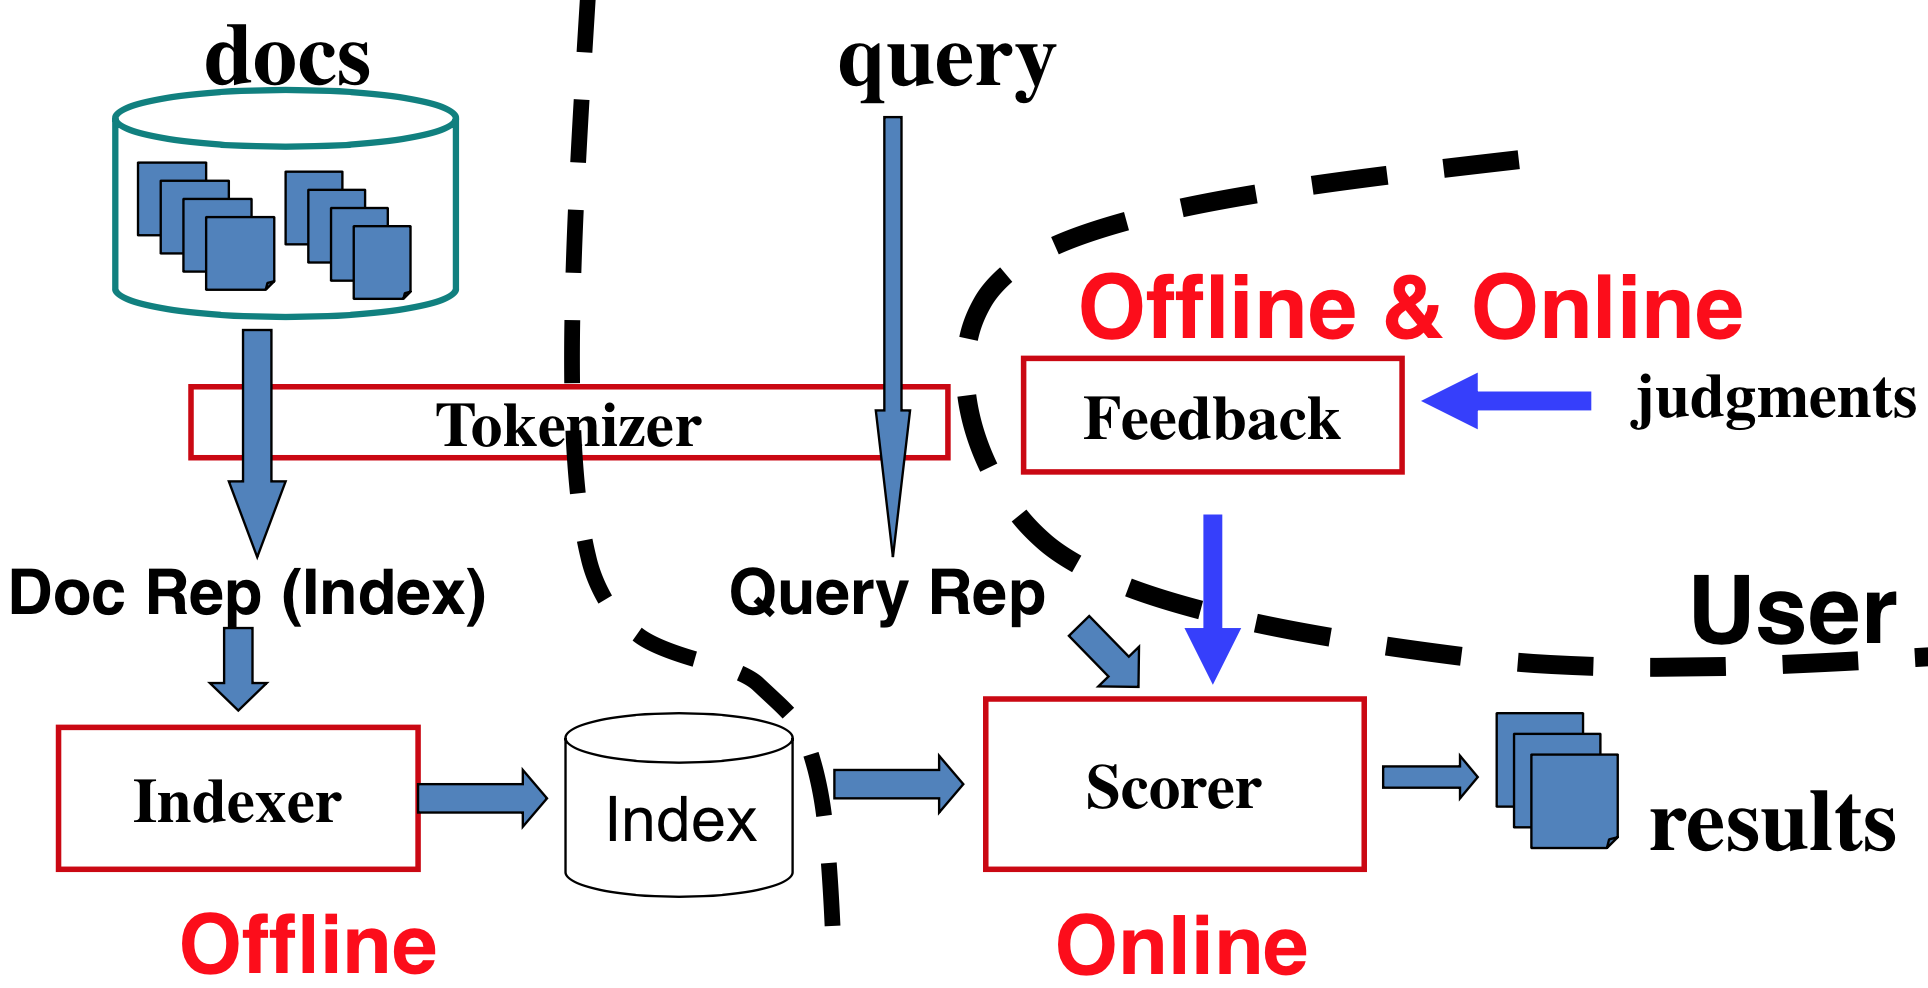
\includegraphics[width=0.75\linewidth]{TR_architecture.png}
\end{figure}

%----------------------------------------
\subsubsection{Tokenization}
\begin{itemize}
\item Normalize lexical units: words with similar meanings should be mapped to the same indexing term
\item Stemming: mapping all inflectional forms of words to the same root form
\item Some languages (e.g., Chinese) pose challenges in word segmentation
\end{itemize}

%----------------------------------------
\subsubsection{Inverted Index}
\begin{figure}[H]
    \centering
    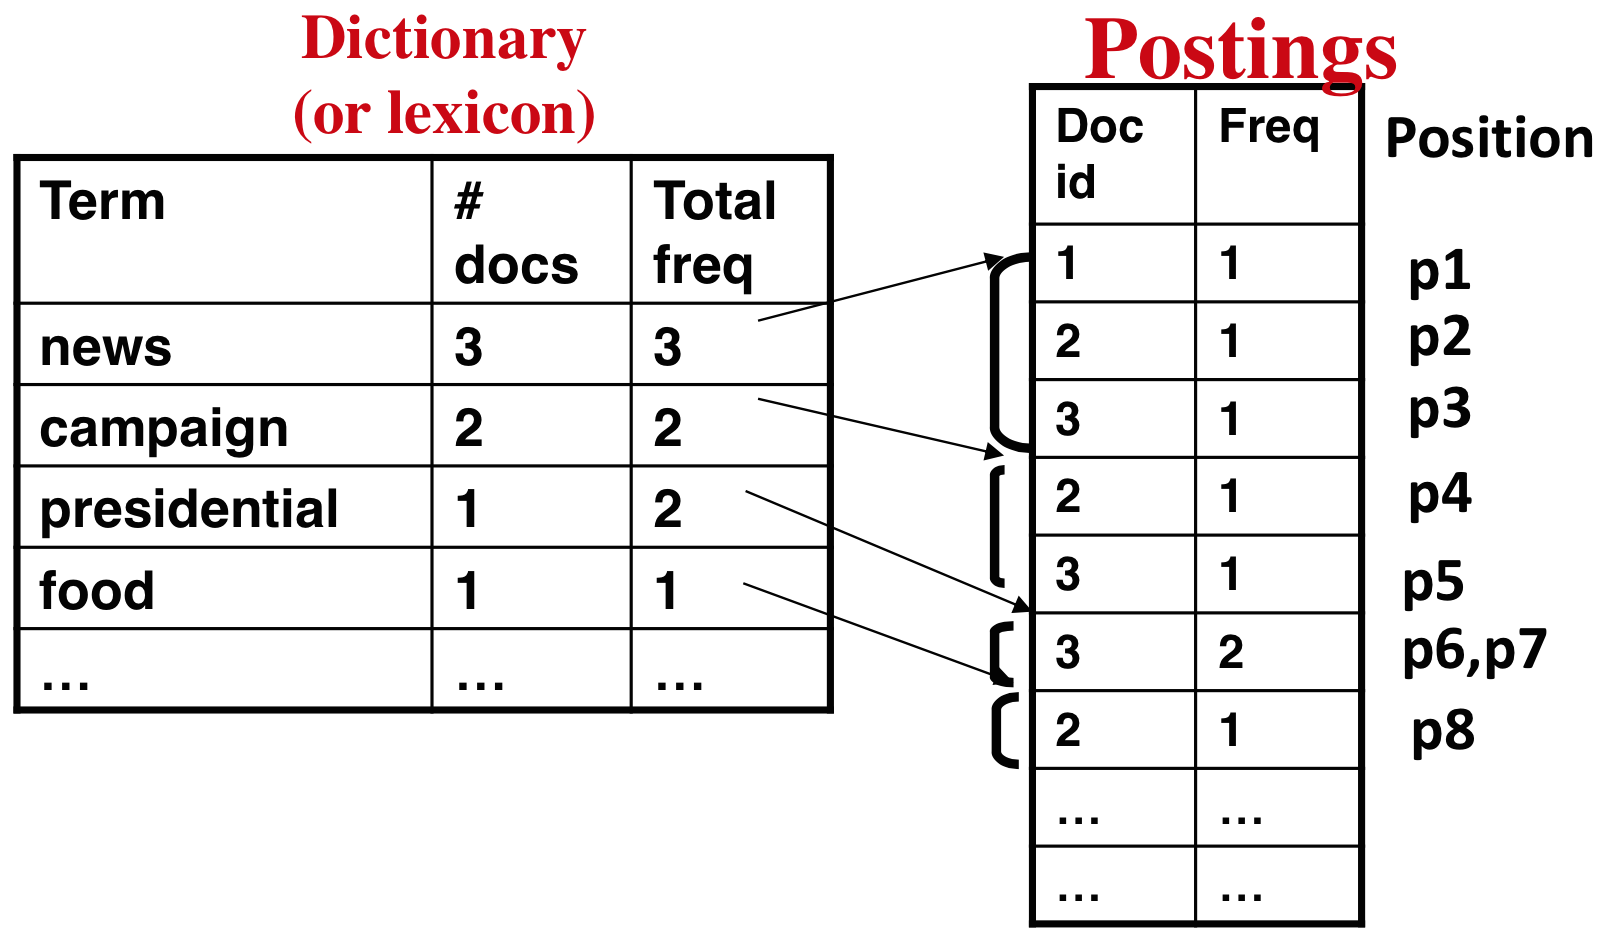
\includegraphics[width=0.5\linewidth]{inverted_index.png}
\end{figure}


%----------------------------------------
\subsubsection{Empirical Distribution of Words}
There are stable language-independent patterns in how people use natural languages:
\begin{itemize}
\item A few words occur very frequently; most occur rarely. E.g., in news articles:
\begin{itemize}
\item Top 4 words: 10~15\% word occurrences 
\item Top 50 words: 35~40\% word occurrences
\end{itemize}
\item The most frequent word in one corpus may be rare in another
\end{itemize}


%----------------------------------------
\subsubsection{Zipf’s Law}
\begin{figure}[H]
    \centering
    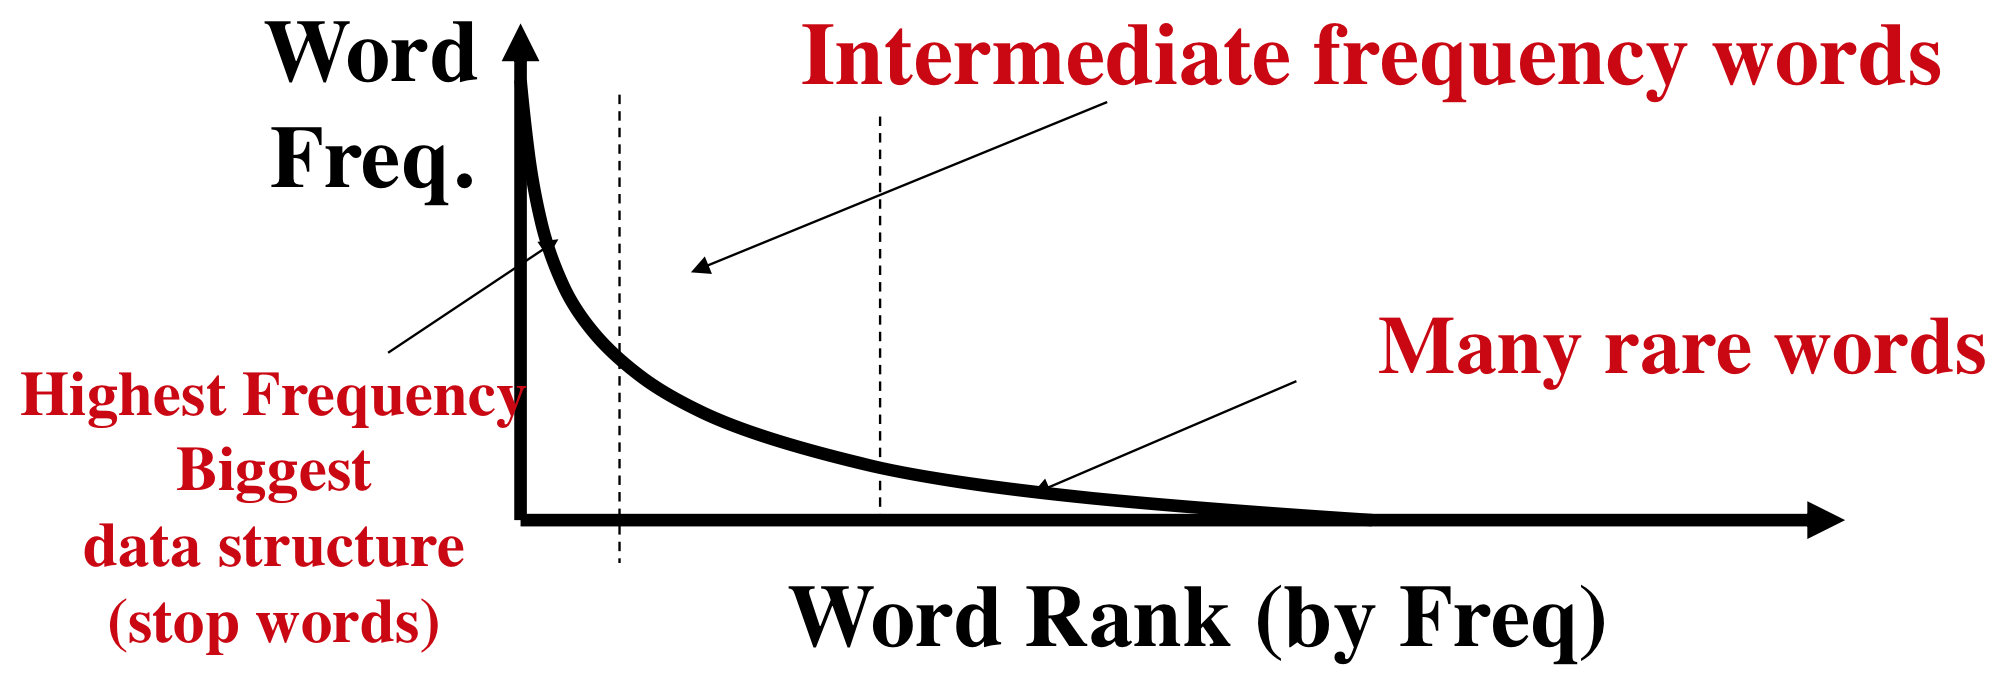
\includegraphics[width=0.95\linewidth]{zipf_law.png}
\end{figure}

\begin{equation*}
F(w) = \frac{C}{r(w)^\alpha}, \alpha \approx 1, C \approx 0.1
\end{equation*}
$\textrm{rank} \times \textrm{frequency} \approx \textrm{constant}$:
\begin{itemize}
\item $F(w)$ - word frequency
\item $r(w)$ - word rank
\end{itemize}


%----------------------------------------
\subsubsection{Data Structures for Inverted Index}
\begin{itemize}
\item Dictionary: modest size
\begin{itemize}
\item Needs fast random access 
\item Preferred to be in memory 
\item Hash table, B-tree, trie, ...
\end{itemize}

\item Postings: huge
\begin{itemize}
\item Sequential access is expected
\item Can stay on disk
\item May contain docID, term freq., term pos, etc 
\item Compression is desirable
\end{itemize}
\end{itemize}

%----------------------------------------
\subsection{Inverted Index Construction}

Sort-based method:
\begin{itemize}
\item Step 1: Collect local (termID, docID, freq) tuples from documents
\item Step 2: Sort local tuples by termID (to make <<runs>>) and save to files
\item Step 3: Pair-wise merge runs
\item Step 4: Output inverted file
\end{itemize}


%----------------------------------------
\subsubsection{Inverted Index Compression}

In general, leverage skewed distribution of values and use variable-length encoding:
\begin{itemize}
\item TF compression:
\begin{itemize}
\item Small numbers tend to occur far more frequently than large
numbers (Zipf's law)
\item Fewer bits for small (high frequency) integers at the cost of more bits for large integers
\end{itemize}

\item Doc ID compression:
\begin{itemize}
\item <<d-gap>> (store difference): $d_1, d_2-d_1, d_3-d_2, \dots$
\item Feasible due to sequential access
\end{itemize}
\end{itemize}

%----------------------------------------
\subsubsection{Integer Compression Methods}
\begin{itemize}
\item \textbf{Binary}: equal-length coding
\item \textbf{Unary}: $x \geqslant 1$ is coded as $x-1$ one bits followed by 0, e.g.,
3=> 110; 5=>11110
\item \textbf{$\gamma$-code}: x => unary code for $1+\lfloor \log x \rfloor$ followed by uniform code for $x-2^{\lfloor \log x \rfloor}$ in $\lfloor \log x \rfloor$ bits, e.g., 3=>101, 5=>11001
\item \textbf{$\delta$-code}: same as $\gamma$-code, but replace the unary prefix with $\gamma$-code. E.g., 3=>1001, 5=>10101
\end{itemize}

%----------------------------------------
\subsection{Fast Search}
\subsubsection{General Form of Scoring Function}
\begin{equation*}
f(q,d) = f_a\left( h\left( g(t_1, d, q), \dots, g(t_k, d, q)\right), f_d(d), f_q(q)\right)
\end{equation*}
\begin{itemize}
\item $f_d(d), f_q(q)$ - adjustment factors of document and query
\item $g(t_i, d, q)$ - weight of a \textbf{matched} query term $t_i$ in $d$
\item $h()$ - weights aggregation function 
\item $f_a()$ - final score adjustment function
\end{itemize}


%----------------------------------------
\subsubsection{A General Algorithm for Ranking Documents}
\begin{itemize}
\item $f_d(d)$ - can be precomputed at index time, $f_q(q)$ - at query time
\item Maintain a score accumulator for each $d$ to compute $h$

\item For each query term $t_i$
\begin{itemize}
\item Fetch the inverted list $\{(d_1,f_1),\dots ,(d_n,f_n)\}$
\item For each entry $(d_j,f_j)$, compute $g(t_i,d_j,q)$, and update score accumulator for doc $d_i$ to incrementally compute $h$
\end{itemize}
\item Adjust the score to compute $f_a$, and sort
\end{itemize}


%----------------------------------------
\subsubsection{Further Improving Efficiency}
\begin{itemize}
\item Caching (e.g., query results, list of inverted index)
\item Keep only the most promising accumulators
\item Scaling up to the Web-scale? (need parallel processing)
\end{itemize}


%----------------------------------------
\subsection{Some Text Retrieval Toolkits}
\begin{itemize}
\item \href{http://lucene.apache.org/}{Lucene}
\item \href{http://www.lemurproject.org/}{Lemur/Indri}
\item \href{http://terrier.org/}{Terrier}
\item \href{http://meta-toolkit.github.io/meta/}{MeTA}
\item More can be found \href{http://timan.cs.uiuc.edu/resources}{here}
\end{itemize}


%----------------------------------------
\subsection{Summary of System Implementation}
\begin{itemize}
\item Inverted index and its construction 
\begin{itemize}
\item Preprocess data as much as we can 
\item Compression when appropriate
\end{itemize}

\item Fast search using inverted index
\begin{itemize}
\item Exploit inverted index to accumulate scores for documents matching
a query term
\item Exploit Zipf’s law to avoid touching many documents not matching any query term
\item Can support a wide range of ranking algorithms
\end{itemize}

\item Further scaling up using distributed file system, parallel processing, and caching
\end{itemize}


%----------------------------------------
\subsection{Recommended reading}
\begin{itemize}
\item Ian H. Witten, Alistair Moffat, Timothy C. Bell: <<Managing Gigabytes: Compressing and Indexing Documents and Images>>, Second Edition. Morgan Kaufmann, 1999.
\item Stefan B{\"u}ttcher, Charles L. A. Clarke, Gordon V. Cormack: <<Information Retrieval - Implementing and Evaluating Search Engines>>. MIT Press, 2010.
\end{itemize}
